\section{Modelación de la planta}
\begin{figure}[ht]
  \begin{center}
    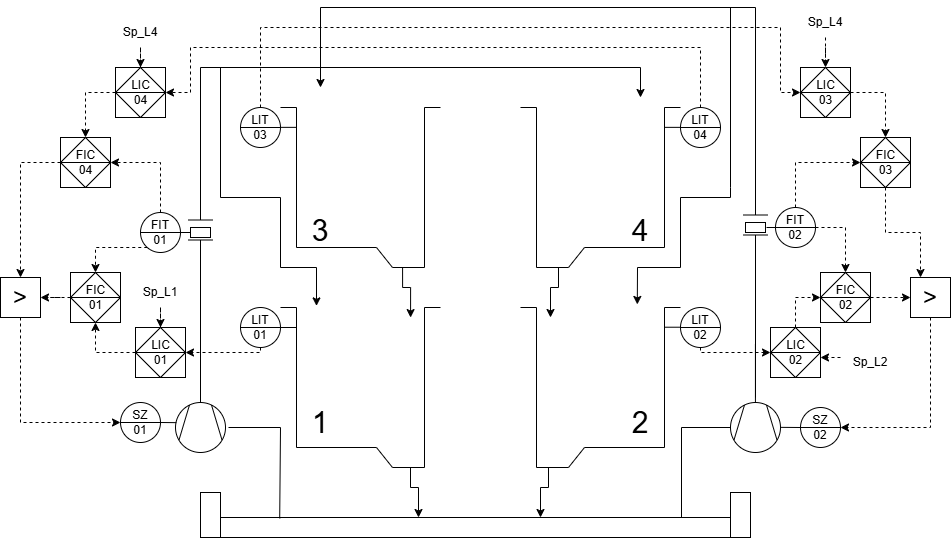
\includegraphics[width=0.95\textwidth]{img/planta_4_estanques_P&ID.png}
  \end{center}
  \caption{P\&ID de la planta de 4 estanques}\label{fig:p&id}
\end{figure}

\clearpage

\subsection{Parámetros del Sistema}

Para el desarrollo del modelo fenomenológico y las posteriores estrategias de control, se definen los parámetros físicos de la planta de 4 estanques. Los valores presentados en la Tabla \ref{tab:parametros} corresponden a las dimensiones físicas de los depósitos, las características de los actuadores y las constantes operativas del controlador ControlLogix.

Es imperativo destacar que el correcto levantamiento de estos parámetros es fundamental, ya que el algoritmo de prealimentación (Feed-Forward) invierte el modelo físico basándose estrictamente en estas magnitudes.

\begin{table}[ht]
    \centering
    \caption{Parámetros físicos y operativos de la Planta de 4 Estanques}
    \label{tab:parametros}
    \renewcommand{\arraystretch}{1.2} % Mejora el espaciado de las filas
    \begin{tabular}{llcc}
        \hline
        \textbf{Símbolo} & \textbf{Descripción} & \textbf{Valor} & \textbf{Unidad} \\
        \hline
        $A_1, A_3$ & Área transversal de los estanques impares & 0.159 & $m^2$ \\
        $A_2, A_4$ & Área transversal de los estanques pares & 0.159 & $m^2$ \\
        $a_1$ & Área del orificio de descarga (estanque 1) &  6.1360e-4 & $m^2$ \\
        $a_2$ & Área del orificio de descarga (estanque 2) & 5.4678e-4  & $m^2$ \\
        $a_3$ & Área del orificio de descarga (estanque 3) &  3.5752e-4 & $m^2$ \\
        $a_4$ & Área del orificio de descarga (estanque 4) &  4.1820e-4 & $m^2$ \\
        $k_1$ & Ganancia de la Bomba 1 (Variador 1) & 0.0017 & $(m^3/s)$ \\
        $k_2$ & Ganancia de la Bomba 2 (Variador 2) & 0.0017 & $(m^3/s)$ \\
        $\gamma_1$ & Fracción de flujo de la válvula de 3 vías (Bomba 1) & 0.455 & Adimensional \\
        $\gamma_2$ & Fracción de flujo de la válvula de 3 vías (Bomba 2) & 0.415 & Adimensional \\
        $g$ & Aceleración de la gravedad & 9.81 & $m/s^2$ \\
        $T_s$ & Tiempo de muestreo & 0.1 & $s$ \\
        \hline
    \end{tabular}
\end{table}

\clearpage
\subsection{Balance de Masas} % Ecuaciones diferenciales

El modelo fenomenológico de la planta se obtiene aplicando el principio de conservación de masa para cada depósito. La variación de volumen en el tiempo ($\frac{dV}{dt} = A \frac{dh}{dt}$) es igual a la suma de los caudales que ingresan menos los caudales que salen. 

Utilizando la Ley de Torricelli para modelar la descarga por gravedad a través de los orificios, la dinámica no lineal del sistema de cuatro estanques queda descrita por el siguiente conjunto de Ecuaciones Diferenciales Ordinarias (EDO):

\begin{align}
    A_1 \frac{dh_1}{dt} &= -a_1 \sqrt{2g h_1} + a_3 \sqrt{2g h_3} + \gamma_1 k_1 f_1 \label{eq:edo_h1} \\
    A_2 \frac{dh_2}{dt} &= -a_2 \sqrt{2g h_2} + a_4 \sqrt{2g h_4} + \gamma_2 k_2 f_2 \label{eq:edo_h2} \\
    A_3 \frac{dh_3}{dt} &= -a_3 \sqrt{2g h_3} + (1-\gamma_2) k_2 f_2 \label{eq:edo_h3} \\
    A_4 \frac{dh_4}{dt} &= -a_4 \sqrt{2g h_4} + (1-\gamma_1) k_1 f_1 \label{eq:edo_h4}
\end{align}

Donde la variable $h_i$ representa el nivel del estanque $i$, y $f_j$ corresponde a la señal de control aplicada a la bomba $j$. Los términos proporcionales a $\gamma$ y $(1-\gamma)$ reflejan la división del caudal en las válvulas.

\subsection{Discretización} % Euler

Para implementar las estrategias de control y realizar simulaciones computacionales, es necesario transformar el modelo continuo a su equivalente en tiempo discreto. Dado que los tiempos de muestreo ($T_s$) típicamente utilizados en la automatización de procesos industriales son pequeños en comparación con la constante de tiempo dominante de los estanques, el método de integración de Euler hacia adelante resulta suficiente y computacionalmente eficiente para el autómata.

Aproximando la derivada del nivel como la tasa de cambio entre dos instantes de muestreo consecutivos:
\begin{equation}
    \frac{dh(t)}{dt} \approx \frac{h[k+1] - h[k]}{T_s}
\end{equation}

Reemplazando esta aproximación en el balance de masas, se obtiene el sistema de ecuaciones en diferencias que predice el nivel en el instante futuro $[k+1]$ basándose en el estado actual $[k]$ y la acción de control actual $u[k]$:

\begin{align}
    h_1[k+1] &= h_1[k] + \frac{T_s}{A_1} \left( -a_1 \sqrt{2g h_1[k]} + a_3 \sqrt{2g h_3[k]} + \gamma_1 k_1 u_1[k] \right) \label{eq:disc_h1} \\
    h_2[k+1] &= h_2[k] + \frac{T_s}{A_2} \left( -a_2 \sqrt{2g h_2[k]} + a_4 \sqrt{2g h_4[k]} + \gamma_2 k_2 u_2[k] \right) \label{eq:disc_h2} \\
    h_3[k+1] &= h_3[k] + \frac{T_s}{A_3} \left( -a_3 \sqrt{2g h_3[k]} + (1-\gamma_2) k_2 u_2[k] \right) \label{eq:disc_h3} \\
    h_4[k+1] &= h_4[k] + \frac{T_s}{A_4} \left( -a_4 \sqrt{2g h_4[k]} + (1-\gamma_1) k_1 u_1[k] \right) \label{eq:disc_h4}
\end{align}

Estas ecuaciones discretas son la base tanto para la simulación de la planta en software externo como para la posterior deducción de los algoritmos de control digital implementados en el PLC.

\subsection{Modelo del Sistema}
\subsubsection{Linealización}
Tomando las ecuaciones \ref{eq:edo_h1}, \ref{eq:edo_h2}, \ref{eq:edo_h3} y \ref{eq:edo_h4}. Se aplica una aproximación de \textbf{Taylor} de primer orden, alrededor de los niveles en estado estacionario $(h_i^0, Q_{in}^0)$, definimos la función de descarga:

\begin{equation}
f(h_i) = a_i \sqrt{2g h_i} = a_i \sqrt{2g} \cdot h_i^{1/2}
\label{eq:func_descarga}
\end{equation}

Se aplica la expansión en Series de Taylor truncada al primer orden alrededor de $h_i^0$:

\begin{equation}
f(h_i) \approx f(h_i^0) + \left. \frac{df(h_i)}{dh_i} \right|_{h_i = h_i^0} (h_i - h_i^0)
\label{eq:taylor_exp}
\end{equation}

Se calcula la primera derivada de la función con respecto a $h_i$:

\begin{equation}
\frac{df(h_i)}{dh_i} = a_i \sqrt{2g} \left( \frac{1}{2} h_i^{-1/2} \right) = \frac{a_i \sqrt{2g}}{2\sqrt{h_i}}
\label{eq:derivada_f}
\end{equation}

Evaluando la derivada estrictamente en el punto de operación $h_i^0$ y reescribiendo algebraicamente para agrupar términos en la raíz:

\begin{equation}
\left. \frac{df(h_i)}{dh_i} \right|_{h_i = h_i^0} = \frac{a_i \sqrt{2g}}{\sqrt{4 h_i^0}} = a_i \sqrt{\frac{2g}{4 h_i^0}} = a_i \sqrt{\frac{g}{2 h_i^0}}
\label{eq:derivada_eval}
\end{equation}

Sustituyendo \eqref{eq:derivada_eval} en \eqref{eq:taylor_exp}, la aproximación lineal del flujo de salida es:

\begin{equation}
Q_{out} \approx a_i \sqrt{2g h_i^0} + \left( a_i \sqrt{\frac{g}{2 h_i^0}} \right) (h_i - h_i^0)
\label{eq:qout_aprox}
\end{equation}

\subsection{Variables de Desviación y Modelo LTI}
Se definen las variables de desviación respecto al punto de equilibrio:
\begin{align*}
\Delta h_i(t) &= h_i(t) - h_i^0 \\
\Delta Q_{in}(t) &= Q_{in}(t) - Q_{in}^0
\end{align*}

Reemplazando la aproximación \eqref{eq:qout_aprox} y las variables de desviación en la ecuación diferencial original, y sabiendo que en estado estacionario $Q_{in}^0 = a_i \sqrt{2g h_i^0}$ (por lo que se anulan), se obtiene:

\begin{equation}
A_i \frac{d(\Delta h_i(t))}{dt} = \Delta Q_{in}(t) - \left( a_i \sqrt{\frac{g}{2 h_i^0}} \right) \Delta h_i(t)
\label{eq:edo_desviacion}
\end{equation}

Dividiendo la expresión por el área del estanque $A_i$ para normalizar la derivada:

\begin{equation}
\frac{d(\Delta h_i(t))}{dt} = - \left( \frac{a_i}{A_i} \sqrt{\frac{g}{2 h_i^0}} \right) \Delta h_i(t) + \frac{1}{A_i} \Delta Q_{in}(t)
\label{eq:edo_normalizada}
\end{equation}

\subsection{Definición de la Constante de Tiempo ($T_i$)}
La ecuación \eqref{eq:edo_normalizada} corresponde a la forma canónica de un sistema lineal de primer orden LTI (Linear Time-Invariant):

\begin{equation}
\frac{dx(t)}{dt} = -\frac{1}{T} x(t) + K u(t)
\label{eq:lti_canonica}
\end{equation}

Por inspección directa entre las ecuaciones \eqref{eq:edo_normalizada} y \eqref{eq:lti_canonica}, se puede notar que el término recíproco de la constante de tiempo $T_i$ es:

\begin{equation}
\frac{1}{T_i} = \frac{a_i}{A_i} \sqrt{\frac{g}{2 h_i^0}}
\label{eq:ti_inversa}
\end{equation}

Despejando $T_i$, aparece la expresión final documentada en el modelo de Johansson \cite{johansson2000}:

\begin{equation}
T_i = \frac{A_i}{a_i} \sqrt{\frac{2 h_i^0}{g}}
\label{eq:ti_final}
\end{equation}

Esta deducción demuestra analíticamente que la inercia dinámica del sistema ($T_i$) no es constante, sino que depende de manera no lineal del nivel del líquido en el punto de operación $h_i^0$.

\subsection{Matriz de Transferencia y Análisis de Ceros de Transmisión}

Una vez obtenidas las constantes de tiempo ($T_i$) mediante la linealización de la Ley de Torricelli por Series de Taylor, es posible representar la dinámica completa de la Planta de Cuatro Estanques de Johansson en el dominio de la frecuencia. Este análisis revelará la influencia estructural de las válvulas de tres vías ($\gamma_1, \gamma_2$) sobre la naturaleza de la fase del sistema multivariable.

\subsubsection{Representación en el Dominio de Laplace}
Considerando que la planta física está construida con cilindros de dimensiones idénticas, se asume un área transversal uniforme tal que $A_1 = A_2 = A_3 = A_4 = A$. Bajo esta premisa, las razones de área se anulan ($\frac{A_i}{A_j} = 1$), simplificando el sistema de ecuaciones diferenciales a:

\begin{align}
\frac{dx_1}{dt} &= -\frac{1}{T_1} x_1 + \frac{1}{T_3} x_3 + \frac{\gamma_1 k_1}{A} u_1 \label{eq:dx1_dt_simp} \\
\frac{dx_2}{dt} &= -\frac{1}{T_2} x_2 + \frac{1}{T_4} x_4 + \frac{\gamma_2 k_2}{A} u_2 \label{eq:dx2_dt_simp} \\
\frac{dx_3}{dt} &= -\frac{1}{T_3} x_3 + \frac{(1-\gamma_2) k_2}{A} u_2 \label{eq:dx3_dt_simp} \\
\frac{dx_4}{dt} &= -\frac{1}{T_4} x_4 + \frac{(1-\gamma_1) k_1}{A} u_1 \label{eq:dx4_dt_simp}
\end{align}

Aplicando la Transformada de Laplace bajo condiciones iniciales nulas, y resolviendo para los estanques superiores (3 y 4), se obtiene:

\begin{align}
X_3(s) &= \frac{(1-\gamma_2) k_2 T_3 / A}{1 + sT_3} U_2(s) \label{eq:X3_s} \\
X_4(s) &= \frac{(1-\gamma_1) k_1 T_4 / A}{1 + sT_4} U_1(s) \label{eq:X4_s}
\end{align}

Sustituyendo \eqref{eq:X3_s} en la ecuación transformada del Estanque 1, y \eqref{eq:X4_s} en la del Estanque 2, se derivan las ecuaciones de los estanques maestros:

\begin{align}
X_1(s) &= \left( \frac{c_1 \gamma_1}{1 + sT_1} \right) U_1(s) + \left( \frac{c_1 (1-\gamma_2)}{(1+sT_1)(1+sT_3)} \right) U_2(s) \label{eq:X1_s} \\
X_2(s) &= \left( \frac{c_2 (1-\gamma_1)}{(1+sT_2)(1+sT_4)} \right) U_1(s) + \left( \frac{c_2 \gamma_2}{1 + sT_2} \right) U_2(s) \label{eq:X2_s}
\end{align}

Donde $c_1 = \frac{T_1 k_1}{A}$ y $c_2 = \frac{T_2 k_2}{A}$.

\subsubsection{Matriz de Transferencia $G(s)$}
El sistema MIMO (Múltiples Entradas, Múltiples Salidas) se define matricialmente como $X(s) = G(s)U(s)$:

\begin{equation}
G(s) = \begin{bmatrix} 
\frac{c_1 \gamma_1}{1 + sT_1} & \frac{c_1 (1-\gamma_2)}{(1+sT_1)(1+sT_3)} \\ 
\frac{c_2 (1-\gamma_1)}{(1+sT_2)(1+sT_4)} & \frac{c_2 \gamma_2}{1 + sT_2} 
\end{bmatrix}
\label{eq:matriz_Gs}
\end{equation}

Se observa que la diagonal principal rige la dinámica directa (primer orden), mientras que la anti-diagonal gobierna el acoplamiento cruzado (segundo orden).

\subsubsection{Cálculo de los Ceros de Transmisión Multivariables}
En un sistema MIMO cuadrado ($2 \times 2$), los ceros de transmisión corresponden a las raíces del polinomio resultante de igualar el determinante de la matriz de transferencia a cero:

\begin{equation}
\det(G(s)) = G_{11}G_{22} - G_{12}G_{21} = 0
\label{eq:det_Gs}
\end{equation}

Sustituyendo los elementos de la matriz y factorizando el término común $\frac{c_1 c_2}{(1+sT_1)(1+sT_2)}$:

\begin{equation}
\frac{c_1 c_2}{(1+sT_1)(1+sT_2)} \left[ \gamma_1 \gamma_2 - \frac{(1-\gamma_1)(1-\gamma_2)}{(1+sT_3)(1+sT_4)} \right] = 0
\label{eq:ceros_factorizado}
\end{equation}

Para encontrar los ceros, igualamos el término entre corchetes a cero y se multiplica por el denominador $(1+sT_3)(1+sT_4)$:

\begin{equation}
\gamma_1 \gamma_2 (1+sT_3)(1+sT_4) - (1-\gamma_1)(1-\gamma_2) = 0
\label{eq:ecuacion_ceros}
\end{equation}

Expandiendo el producto de las constantes de tiempo y agrupando los coeficientes según el grado de $s$:

\begin{equation}
s^2 [\gamma_1 \gamma_2 T_3 T_4] + s [\gamma_1 \gamma_2 (T_3+T_4)] + (\gamma_1 + \gamma_2 - 1) = 0
\label{eq:polinomio_caracteristico_ceros}
\end{equation}
\clearpage
\subsubsection{Análisis de Estabilidad y Fase del Sistema}
La Ecuación \eqref{eq:polinomio_caracteristico_ceros} es una cuadrática característica de los ceros del sistema. De acuerdo con el criterio de Routh-Hurwitz, para que las raíces se encuentren estrictamente en el Semiplano Izquierdo ($LHP$) de Laplace, todos los coeficientes del polinomio deben poseer el mismo signo positivo.

Dado que $T_3, T_4 > 0$ y $\gamma_1, \gamma_2 \in (0, 1)$, los coeficientes de $s^2$ y $s$ son constitutivamente positivos. Por lo tanto, la ubicación de los ceros depende exclusivamente del término independiente:

\textbf{Condición de Fase Mínima (Ceros LHP):}
Para un comportamiento controlable sin respuesta inversa transitoria, se requiere:
\begin{equation}
\gamma_1 + \gamma_2 - 1 > 0 \implies \gamma_1 + \gamma_2 > 1
\label{eq:condicion_fase_minima}
\end{equation}
Físicamente, esto indica que los flujos directos hacia los estanques inferiores dominan sobre el acoplamiento cruzado hacia los estanques superiores.

\textbf{Condición de Fase No Mínima (Ceros RHP):}
Bajo la configuración asignada al proyecto ($\gamma_1 = 0.455$, $\gamma_2 = 0.4195$), la suma resulta en $0.8745$.
\begin{equation}
\gamma_1 + \gamma_2 - 1 < 0 \implies \gamma_1 + \gamma_2 < 1
\label{eq:condicion_fase_no_minima}
\end{equation}
Esta inecuación \eqref{eq:condicion_fase_no_minima} demuestra que el término independiente es negativo. Según Routh-Hurwitz, la alternancia de signos en el polinomio garantiza la existencia de al menos una raíz en el Semiplano Derecho ($RHP$). Este Cero de Transmisión de Semiplano Derecho provoca matemáticamente el fenómeno de subamortiguación inicial (Undershoot) o Respuesta Inversa, limitando severamente la aplicabilidad de controladores PID de alta ganancia.
\clearpage
\subsection{Cálculo del Punto de Operación y Restricciones Estáticas}

Para determinar la viabilidad de un punto de operación $(h_1^0, h_2^0)$ y calcular los esfuerzos de control requeridos $(u_1^0, u_2^0)$, se debe analizar el sistema en estado estacionario. 

\subsubsection{Balance de Masa en Estado Estacionario}
Con base en las ecuaciones diferenciales no lineales del sistema, en estado estacionario o de equilibrio, no hay acumulación de volumen en los estanques, por lo que las derivadas del nivel con respecto al tiempo se igualan a cero ($\frac{dh_i}{dt} = 0$). 

Esto implica que el flujo volumétrico total que entra a cada estanque es exactamente igual al flujo que sale por gravedad (Ley de Torricelli):

\begin{align}
\text{Estanque 1:} \quad a_1 \sqrt{2g h_1^0} &= \gamma_1 k_1 u_1^0 + a_3 \sqrt{2g h_3^0} \label{eq:estatico_1} \\
\text{Estanque 2:} \quad a_2 \sqrt{2g h_2^0} &= \gamma_2 k_2 u_2^0 + a_4 \sqrt{2g h_4^0} \label{eq:estatico_2} \\
\text{Estanque 3:} \quad a_3 \sqrt{2g h_3^0} &= (1-\gamma_2) k_2 u_2^0 \label{eq:estatico_3} \\
\text{Estanque 4:} \quad a_4 \sqrt{2g h_4^0} &= (1-\gamma_1) k_1 u_1^0 \label{eq:estatico_4}
\end{align}

\subsubsection{Reducción del Sistema por Sustitución}
El objetivo es encontrar una relación directa entre los actuadores ($u_1, u_2$) y los niveles de los estanques maestros inferiores ($h_1, h_2$). 

Observando las ecuaciones \eqref{eq:estatico_3} y \eqref{eq:estatico_4}, notamos que los términos de descarga de los estanques superiores ($a_3 \sqrt{2g h_3^0}$ y $a_4 \sqrt{2g h_4^0}$) dependen de manera directa y lineal de los comandos de las bombas cruzadas.

Sustituyendo la ecuación \eqref{eq:estatico_3} en la ecuación \eqref{eq:estatico_1}:
\begin{equation}
a_1 \sqrt{2g h_1^0} = \gamma_1 k_1 u_1^0 + (1-\gamma_2) k_2 u_2^0
\label{eq:reducida_1}
\end{equation}

Sustituyendo la ecuación \eqref{eq:estatico_4} en la ecuación \eqref{eq:estatico_2}:
\begin{equation}
a_2 \sqrt{2g h_2^0} = (1-\gamma_1) k_1 u_1^0 + \gamma_2 k_2 u_2^0
\label{eq:reducida_2}
\end{equation}

\subsubsection{Representación Matricial (Matriz Estática)}
Para simplificar la notación, definimos los "Flujos de Fuga Deseados" en los estanques inferiores como constantes dependientes de los Setpoints:
\begin{align*}
F_1 &= a_1 \sqrt{2g h_1^0} \\
F_2 &= a_2 \sqrt{2g h_2^0}
\end{align*}

Reescribiendo las ecuaciones \eqref{eq:reducida_1} y \eqref{eq:reducida_2} en forma matricial, se obtiene la relación lineal que mapea los esfuerzos de control con los flujos de descarga en estado estacionario:

\begin{equation}
\begin{bmatrix} F_1 \\ F_2 \end{bmatrix} = 
\underbrace{
\begin{bmatrix} 
\gamma_1 k_1 & (1-\gamma_2) k_2 \\ 
(1-\gamma_1) k_1 & \gamma_2 k_2 
\end{bmatrix}
}_{M}
\begin{bmatrix} u_1^0 \\ u_2^0 \end{bmatrix}
\label{eq:matriz_estatica}
\end{equation}

Donde $M$ es la Matriz de Ganancia Estática del sistema.

\subsubsection{Cálculo de Actuadores y Restricciones}
Para encontrar los valores requeridos en las bombas para alcanzar un par de niveles $(h_1^0, h_2^0)$, se multiplica por la matriz inversa $M^{-1}$:

\begin{equation}
\begin{bmatrix} u_1^0 \\ u_2^0 \end{bmatrix} = M^{-1} \begin{bmatrix} F_1 \\ F_2 \end{bmatrix}
\label{eq:calculo_bombas}
\end{equation}

Dado que los actuadores tienen restricciones físicas irreducibles ($0 \le u_i \le 1.0$), cualquier vector de flujos $\begin{bmatrix} F_1 & F_2 \end{bmatrix}^T$ que requiera valores de $u$ fuera de este rango se considera un punto de operación físicamente inalcanzable.


\subsubsection{Ecuaciones Base según la Topología}
Siguiendo la arquitectura física de la planta, se establece el origen del agua para cada estanque en estado estacionario:

\begin{align}
F_4 &= (1-\gamma_1) k_1 u_1 \quad \text{(El estanque 4 solo depende de la Bomba 1)} \label{eq:F4_u1} \\
F_3 &= (1-\gamma_2) k_2 u_2 \quad \text{(El estanque 3 solo depende de la Bomba 2)} \label{eq:F3_u2} \\
F_1 &= \gamma_1 k_1 u_1 + F_3 \quad \text{(El estanque 1 recibe de la Bomba 1 y del Estanque 3)} \label{eq:F1_dependencia} \\
F_2 &= \gamma_2 k_2 u_2 + F_4 \quad \text{(El estanque 2 recibe de la Bomba 2 y del Estanque 4)} \label{eq:F2_dependencia}
\end{align}

\subsubsection{El Compromiso del Actuador 1}
Al defininir un \textit{Setpoint} fijo para el Estanque 1, $F_1$ se convierte en una constante conocida. 

Sustituyendo \eqref{eq:F3_u2} en \eqref{eq:F1_dependencia}, Se obtiene la ecuación fundamental que vincula a ambas bombas para satisfacer al Estanque 1:
\begin{equation}
F_1 = \gamma_1 k_1 u_1 + (1-\gamma_2) k_2 u_2
\label{eq:vinculo_bombas}
\end{equation}

Despejando el esfuerzo de la Bomba 1 ($u_1$) necesario para mantener este nivel:
\begin{equation}
u_1 = \frac{F_1 - (1-\gamma_2) k_2 u_2}{\gamma_1 k_1}
\label{eq:u1_despejado}
\end{equation}

\textit{Físicamente, esta ecuación demuestra que si la Bomba 2 ($u_2$) inyecta mucha agua al Estanque 3 (que luego cae al Estanque 1), la Bomba 1 ($u_1$) se ve obligada a reducir su esfuerzo para no sobrepasar el Setpoint $F_1$.}

\subsubsection{Los Límites Físicos}
Las bombas tienen límites físicos absolutos: no pueden operar a potencia negativa ni superar el 100\% de su capacidad. Por lo tanto:
\begin{equation*}
0 \le u_1 \le 1.0 \quad \text{(asumiendo $u_1$ normalizado entre 0 y 1)}
\end{equation*}

Aplicando este límite físico a nuestra ecuación \eqref{eq:u1_despejado}:
\begin{equation}
0 \le \frac{F_1 - (1-\gamma_2) k_2 u_2}{\gamma_1 k_1} \le 1.0
\end{equation}

Al despejar $u_2$ de esta inecuación doble, es evidente que la simple exigencia de mantener el Estanque 1 obliga a la Bomba 2 a operar dentro de un rango cerrado:

\textbf{Límite por apagado de Bomba 1 ($u_1 \ge 0$):}
\begin{equation}
u_2 \le \frac{F_1}{(1-\gamma_2)k_2}
\label{eq:u2_maximo}
\end{equation}

\textbf{Límite por saturación de Bomba 1 ($u_1 \le 1.0$):}
\begin{equation}
u_2 \ge \frac{F_1 - \gamma_1 k_1}{(1-\gamma_2)k_2}
\label{eq:u2_minimo}
\end{equation}

\textit{Conclusión intermedia: Al fijar $h_1$, la Bomba 2 pierde su libertad total de [0 a 100\%] y queda atrapada entre estos dos valores.}

\subsubsection{Repercusión en el Estanque 2 (El Rango Válido)}
Finalmente, tomando la ecuación base \eqref{eq:F2_dependencia} y Sustituyendo $F_4$ usando \eqref{eq:F4_u1}:
\begin{equation}
F_2 = \gamma_2 k_2 u_2 + (1-\gamma_1) k_1 u_1
\end{equation}

Para ver la dependencia total, se sustituye $u_1$ usando la ecuación \eqref{eq:u1_despejado}:
\begin{equation}
F_2 = \gamma_2 k_2 u_2 + (1-\gamma_1) k_1 \left[ \frac{F_1 - (1-\gamma_2) k_2 u_2}{\gamma_1 k_1} \right]
\end{equation}

Simplificando los términos $k_1$ y agrupando lo que multiplica a $F_1$ y lo que multiplica a $u_2$:
\begin{equation}
F_2 = \left( \frac{1-\gamma_1}{\gamma_1} \right) F_1 + \left[ \frac{\gamma_1 \gamma_2 - (1-\gamma_1)(1-\gamma_2)}{\gamma_1} \right] k_2 u_2
\end{equation}

Reduciendo el término entre corchetes, se llega a la ecuación maestra de la planta:
\begin{equation}
F_2 = \underbrace{\left( \frac{1-\gamma_1}{\gamma_1} \right) F_1}_{\text{Constante impuesta por } h_1} + \underbrace{\left( \frac{\gamma_1 + \gamma_2 - 1}{\gamma_1} \right)}_{\text{Pendiente negativa}} k_2 u_2
\label{eq:F2_final}
\end{equation}
\clearpage
